\section{Theory} \label{sec:theory}

\subsection{IPv4}
To navigate the internet, the IP protocol is used. This is mainly split into the popular IPv4 and the new IPv6. IPv4 addresses are 32 bit, meaning they can range from 0.0.0.0 to 255.255.255.255. 

\subsection{IPv6}
IPv6 is an extended version of IPv4, and has has $2^{128}$ unique addresses. IPv6 was 1995, and the plan was to change from using IPv4 to IPv6. However, the global conversion from IPv4 to IPv6 is slow, .While Shodan does support IPv6, most corporations in the maritime and offshore industries are big enough to own IPv4 addresses, and they therefore have little reason to change to IPv6.

\subsection{IP ranges}
 The IPv4 addresses are sold to organisations, for them to distribute further. For example, an Internet Service Provider (ISP) like Telenor will give IPv4 addresses to the customers while they use their subscribed internet connections. This distribution of IPv4 addresses to organisations is illustrated in \cref{fig:ipv4_map}.

\subsubsection{IPv4 exhaustion and NAT}
IPv4 addresses were distributed by the Internet Assigned Numbers Authority (IANA). 11 January, 2011, IANA allocated its last block.\cite{exhasuted_IPV4} Since then, the regional bodies responsible for allocationg IPv4 addresses, Regional Internet Registries (RIR), have also exhausted their IPv4 addresses, the last one in 2019.\cite{exhausted_RIPENNC} Due to this problem, multiple methods are used to get the most out of the IPv4 address space. Arguably, the most popular of these methods are Network Address Translation (NAT). IPv6 was also designed to solve the IPv4 exhaustion challenge.

NAT lets you connect multiple devices to the same IPv4. This is done by using a routing device with a shared IPv4 address to receive packages for multiple different devices, and then redirect the packages to the correct receiver. This makes it so that the devices behind the NAT can reach the internet, while communication from the internet can not reach the devices unless the devices start the communication. This connection is illustrated in \cref{fig:NAT} 


\tikzset{every picture/.style={line width=0.75pt}} %set default line width to 0.75pt        
\begin{tabular}{p{10cm}}
   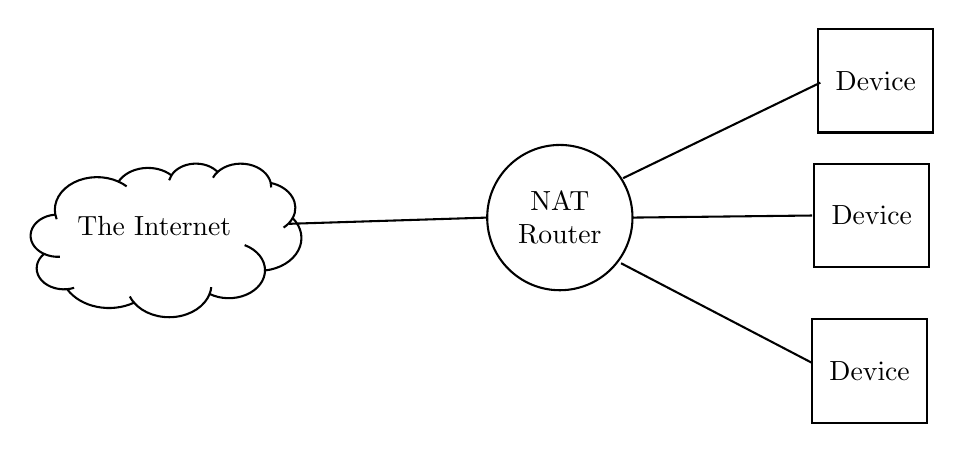
\begin{tikzpicture}[x=0.75pt,y=0.75pt,yscale=-1,xscale=1]
     %uncomment if require: \path (0,300); %set diagram left start at 0, and has height of 300

%Shape: Rectangle [id:dp7550808737565868] 
\draw   (417.5,74) -- (473,74) -- (473,124) -- (417.5,124) -- cycle ;

%Shape: Ellipse [id:dp5744265006375734] 
\draw   (258,165) .. controls (258,145.67) and (273.67,130) .. (293,130) .. controls (312.33,130) and (328,145.67) .. (328,165) .. controls (328,184.33) and (312.33,200) .. (293,200) .. controls (273.67,200) and (258,184.33) .. (258,165) -- cycle ;

%Straight Lines [id:da011152119100300673] 
\draw    (418.5,100) -- (323.5,146) ;
%Shape: Rectangle [id:dp019726233695570805] 
\draw   (414.5,214) -- (470,214) -- (470,264) -- (414.5,264) -- cycle ;

%Shape: Rectangle [id:dp2854982925574172] 
\draw   (415.5,139) -- (471,139) -- (471,189) -- (415.5,189) -- cycle ;

%Straight Lines [id:da042657718924057675] 
\draw    (414.5,164) -- (328,165) ;
%Straight Lines [id:da8590380439733557] 
\draw    (414.5,235) -- (322.5,187) ;
%Shape: Cloud [id:dp5209862047408297] 
\draw   (49.88,163.36) .. controls (48.82,157.4) and (52.27,151.49) .. (58.76,148.15) .. controls (65.25,144.81) and (73.64,144.62) .. (80.36,147.67) .. controls (82.74,144.2) and (87.1,141.8) .. (92.13,141.21) .. controls (97.15,140.61) and (102.24,141.88) .. (105.86,144.64) .. controls (107.89,141.49) and (111.87,139.38) .. (116.4,139.05) .. controls (120.93,138.71) and (125.35,140.21) .. (128.11,143.01) .. controls (131.78,139.67) and (137.61,138.27) .. (143.09,139.4) .. controls (148.57,140.54) and (152.7,144) .. (153.71,148.31) .. controls (158.2,149.25) and (161.95,151.66) .. (163.97,154.91) .. controls (166,158.15) and (166.1,161.92) .. (164.27,165.23) .. controls (168.7,169.68) and (169.73,175.61) .. (166.99,180.8) .. controls (164.25,186) and (158.14,189.68) .. (150.95,190.48) .. controls (150.9,195.35) and (147.44,199.83) .. (141.9,202.17) .. controls (136.37,204.52) and (129.62,204.38) .. (124.26,201.79) .. controls (121.98,207.63) and (115.55,211.93) .. (107.76,212.83) .. controls (99.97,213.73) and (92.21,211.06) .. (87.83,205.99) .. controls (82.46,208.49) and (76.02,209.21) .. (69.96,207.99) .. controls (63.9,206.77) and (58.74,203.7) .. (55.62,199.49) .. controls (50.14,199.99) and (44.84,197.79) .. (42.35,194) .. controls (39.86,190.2) and (40.71,185.61) .. (44.49,182.5) .. controls (39.59,180.28) and (37.1,175.87) .. (38.3,171.56) .. controls (39.5,167.26) and (44.13,164.05) .. (49.76,163.59) ; \draw   (44.49,182.5) .. controls (46.8,183.55) and (49.46,184.03) .. (52.13,183.87)(55.62,199.49) .. controls (56.77,199.39) and (57.89,199.17) .. (58.97,198.84)(87.83,205.99) .. controls (87.02,205.06) and (86.34,204.06) .. (85.81,203.01)(124.26,201.79) .. controls (124.67,200.73) and (124.95,199.63) .. (125.06,198.52)(150.95,190.48) .. controls (151.01,185.28) and (147.19,180.53) .. (141.14,178.26)(164.27,165.23) .. controls (163.29,167) and (161.79,168.57) .. (159.9,169.81)(153.71,148.31) .. controls (153.88,149.02) and (153.95,149.75) .. (153.94,150.47)(128.11,143.01) .. controls (127.2,143.84) and (126.44,144.77) .. (125.87,145.77)(105.86,144.64) .. controls (105.37,145.39) and (105.01,146.19) .. (104.77,147.02)(80.36,147.67) .. controls (81.78,148.31) and (83.1,149.09) .. (84.28,149.97)(49.88,163.36) .. controls (50.02,164.19) and (50.25,165) .. (50.56,165.79) ;

%Straight Lines [id:da9624009852798121] 
\draw    (162.5,168) -- (258,165) ;

% Text Node
\draw (293,165) node   [align=left] {\begin{minipage}[lt]{33.354pt}\setlength\topsep{0pt}
\begin{center}
NAT\\Router
\end{center}

\end{minipage}};
% Text Node
\draw (445.25,99) node   [align=left] {Device};
% Text Node
\draw (442.25,239) node   [align=left] {Device};
% Text Node
\draw (443.25,164) node   [align=left] {Device};
% Text Node
\draw (59,163) node [anchor=north west][inner sep=0.75pt]   [align=left] {The Internet};

   \end{tikzpicture}
   \captionof{figure}{Illustration of a NAT router}
   \label{fig:NAT}
\end{tabular}


\subsubsection{CIDR}
 Classless Inter-Domain Routing(CIDR) is the modern way to split the IPv4 address space into blocks, so that they can be distributed. A CIDR block can look like this: "93.192.0.0/10". This block has two parts, the prefix "93.192.0.0" and the suffix "/10". The prefix indicates the size of the CIDR block. The prefix indicates where in the IPv4 space the CIDR block is located. To understand this, it is useful to look at an IP address in binary instead of decimal. For example, the IPv4 address "93.220.107.30" becomes "01011101.11011100.01101011.00011110". The suffix decides how many bits are fixed. In the CIDR block "93.220.107.30/10", the 10 first bits of the prefix "93.220.107.30"  are "01011101.11xxxxxx.xxxxxxxx.xxxxxxxx". This number span the binary range \\ \{01011101.11111111.11111111.11111111 - 01011101.11000000.00000000.00000000 \}, or the decimal range  \{ 93.192.0.1 - 93.255.255.254 \}. Remark that not the full prefix is needed; "93.220.107.30/10" and "93.220.107.31/10" are the same CIDR  block. Because of this, it is normal to set the changing bits of the prefix to 0, as in: "93.192.0.0/10". 
Since the sizes of CIDR blocks vary, they can be nested. For example, "93.192.0.0/11" is a part of "93.192.0.0/10".


\newpage
